\documentclass[a4paper,12pt]{article}
\usepackage{graphicx} 
\usepackage{geometry}
\usepackage{titlesec} 
\setlength{\parskip}{1em} 
\titleformat{\section}{\normalfont\LARGE\bfseries}{\thesection}{1em}{}
\usepackage{titlesec}
\usepackage{titletoc}
\usepackage{hyperref} 
\geometry{
    top=0.5in,
    bottom=1in, % Adjust the bottom margin,
    headheight=0pt, % Adjust the header height if needed
    footskip=20pt % Adjust footskip to reduce space after page number
}
\usepackage{float}


\begin{document}
\thispagestyle{empty} 
% University logo at the top
\begin{center}
    
\includegraphics[width=0.1\textwidth]{photos/logo.png}  \\[1.5em]
    {\LARGE Noakhali Science \& Technology University} \\
    Department of Computer Science \& Telecommunication Engineering
\end{center}

\vspace{4cm}

% Title of the project report
\begin{center}
    \textbf{\huge Lab Report On:} \\[0.5em]
   \textbf{\LARGE Introduction and Requirement Analysis} \\[1em]
      \textbf{\Large Course Code: CSTE 3210}  \\[1.5em]
    {\large Submitted by:} \\[0.6em]
     \textbf {\large Mohammad Borhan Uddin }  \\
  {\large ID: ASH2101008M}  \\ [0.6em]
    \textbf{\large Mohammad Billal Hossain}  \\
    {\large ID: MUH2101028M}  \\ [2em]

    
    {\large Submitted to:} \\[0.6em]
    \textbf{\large Dr. Nazia Majadi} \\ 
    {\large Associate Professor} \\ 
     {Department of Computer Science \& Telecommunication Engineering} \\ 
\end{center}

\vspace{5cm}

\begin{center}
    \textbf{\LARGE Date : March 12, 2025}
\end{center}
\thispagestyle{empty} 

\tableofcontents

\thispagestyle{empty}
\newpage

\setcounter{page}{1} 

\section{Introduction}

The \textit{Problem Fixer} system is a proposed complaint management platform designed to improve the efficiency of reporting and resolving issues within a university. The system will facilitate structured and transparent handling of complaints, ensuring that problems are addressed in a timely manner.

\subsection{Project Scope}

The \textit{Problem Fixer} system will provide a structured approach for teachers to report issues within the university. These complaints may include malfunctioning office equipment, electrical issues, or sanitation concerns. Complaints will be categorized to ensure efficient handling by the administration. The admin will have the capability to assign employees to specific complaint categories and track resolutions. A notification system will be integrated to update users on the status of their complaints, ensuring smooth communication.

\subsection{Objectives and Goals}

The key objectives and goals of the \textit{Problem Fixer} system include:

\begin{itemize}
\item Developing an \textbf{automated and structured} complaint management system.
\item Allowing \textbf{teachers to submit complaints} and track their progress.
\item Enabling \textbf{administrators to assign employees} to complaints for quick resolution.
\item Ensuring \textbf{timely notifications} through in-system alerts and email updates.
\item Providing users with the ability to \textbf{mark complaints as resolved} once satisfactorily addressed.
\item Improving \textbf{efficiency and accountability} in complaint resolution.
\item Designing the system with \textbf{scalability} to handle increasing users and complaints without performance degradation.
\item Ensuring \textbf{modularity} in the system architecture, allowing easy updates, feature additions, and maintenance.
\item Adhering to \textbf{software engineering best practices}, including clean code, version control, and thorough testing for robust system development.
\end{itemize}


\newpage
\section{Defining Requirements}

This section defines the essential components, functionalities, and performance expectations for the \textit{Problem Fixer} system.

\subsection{System Requirements}

The system will be composed of the following key modules:

\begin{itemize}
\item \textbf{User Module (Teachers):} Enables users to submit complaints, track their status, and mark them as resolved.
\item \textbf{Admin Module:} Allows administrators to manage complaint categories, assign employees, resolve complaints, and send notifications.
\item \textbf{Employee Management Module:} Enables the admin to add employees and assign them to specific complaint categories.
\item \textbf{Notification System:} Sends real-time notifications and emails to users upon complaint updates.
\item \textbf{Database Management:} Securely stores all complaint records, user details, and resolution history.
\end{itemize}

\subsection{Functional Requirements}

The following functionalities will be supported:

\begin{enumerate}
\item \textbf{User Features:}
\begin{itemize}
\item Users can \textbf{log in} and \textbf{submit complaints}.
\item Users can \textbf{select a complaint category} (e.g., Computer, Electrical, Cleaning, AC).
\item Users can \textbf{track the status} of their complaints.
\item Users can \textbf{mark complaints as done} once resolved.
\end{itemize}
\item \textbf{Admin Features:}
\begin{itemize}
    \item Admin can \textbf{log in} and \textbf{manage complaint categories}.
    \item Admin can \textbf{add departments}.
    \item Admin can \textbf{add employees} and \textbf{assign them to specific complaint categories}.
    \item Admin can \textbf{view and manage complaints} submitted by users.
    \item Admin can \textbf{resolve complaints} by providing resolution details.
    \item Admin can \textbf{assign an employee} to handle a complaint if necessary.
    \item Admin can \textbf{send notifications and emails} to users when a complaint is resolved.
\end{itemize}

\end{enumerate}

\subsection{Non-Functional Requirements}

\begin{enumerate}
\item \textbf{Performance Requirements:}
\begin{itemize}
\item The system should be \textbf{scalable and capable of handling multiple complaints concurrently}.
\item Complaint submission and updates should be processed \textbf{in real-time}.
\end{itemize}
\item \textbf{Security Requirements:}
\begin{itemize}
    \item Secure authentication mechanisms must be implemented.
    \item Only \textbf{authorized admins} should be able to manage complaints and assign employees.
\end{itemize}

\item \textbf{Usability Requirements:}
\begin{itemize}
    \item The interface should be \textbf{intuitive and easy to navigate}.
    \item Complaint submission should be \textbf{simple and user-friendly}.
\end{itemize}

\item \textbf{Reliability and Maintainability:}
\begin{itemize}
    \item The system should ensure \textbf{high availability with minimal downtime}.
    \item Data should be \textbf{regularly backed up} to prevent loss.
\end{itemize}
\end{enumerate}
\newpage
\section{Requirement Analysis}

The requirement analysis for the "Problem Fixer" project identifies key system components and user interactions. It focuses on understanding how admins, employees, and teachers interact with the system, automating processes, and managing complaints from submission to resolution. The following use case diagram and descriptions outline the primary system requirements.


\subsection{Scenario-Based Models}

\subsubsection{Use Case Diagram}
The Use Case Diagram for the "Problem Fixer" system models the interactions between the users and the system. The actors in the system include the following.

\begin{itemize}
    \item \textbf{Primary Actor:} User (Teacher) - The individual who submits complaints and marks them as resolved.
    \item \textbf{Secondary Actor:} Admin - The person who manages departments, categories, employees, and resolves complaints.
\end{itemize}
\begin{figure}[H]
    \centering
    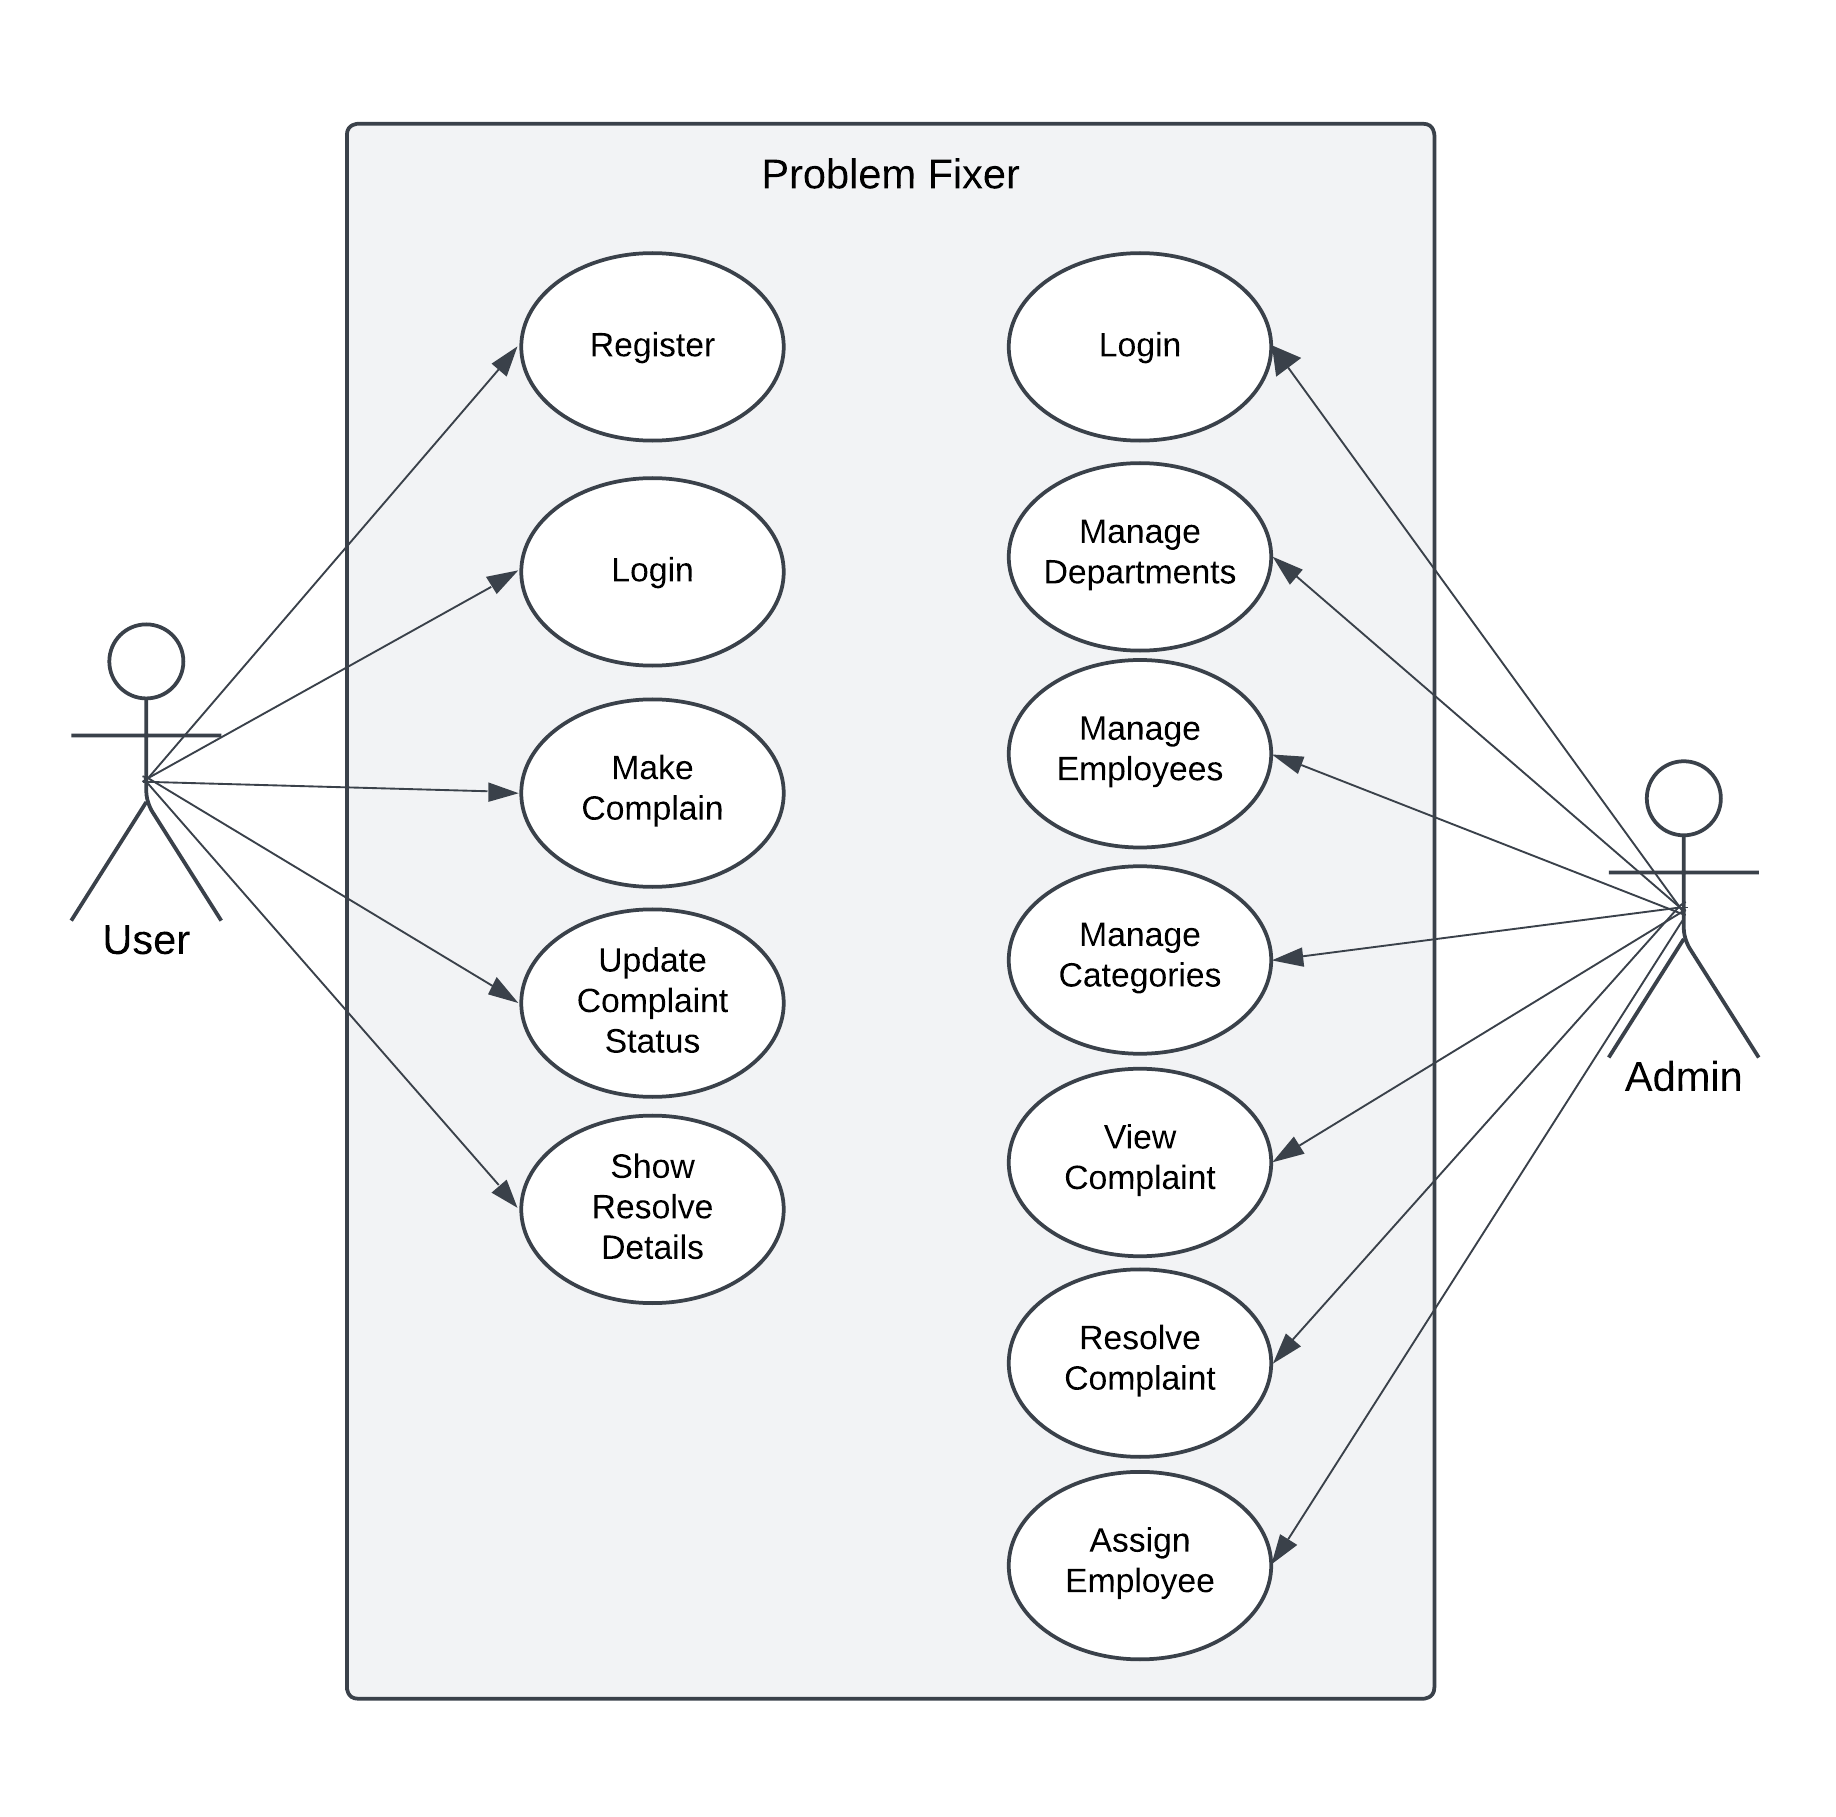
\includegraphics[width=0.85\linewidth]{photos/use-case.png}

    \caption{Use Case Diagram}
    \label{fig:enter-label}
\end{figure}



\subsubsection{Use Case Descriptions}


\textbf{Use Case 1: Submit a Complaint} 
    \begin{itemize}
        \item \textbf{Actor:} User (Teacher)
        \item \textbf{Description:} The user submits a complaint related to a broken item, service request, or facility issue (e.g., a broken office computer). The user selects a category for the complaint (e.g., Computer, Electrical, Cleaning) and provides a description of the issue.
        \item \textbf{Preconditions:} The user is logged into the system.
        \item \textbf{Postconditions:} The complaint is successfully submitted and recorded in the system.
    \end{itemize} 

\noindent \textbf{Use Case 2: Manage Employees, Departments, and Categories}
\begin{itemize}
    \item \textbf{Actor:} Admin
    \item \textbf{Description:} The admin manages employees, departments, and categories to ensure smooth operation of the system. The admin assigns employees to specific departments, creates categories for complaints, and ensures that each department has the appropriate resources to handle complaints efficiently.
    \item \textbf{Preconditions:} The admin is logged into the system and has access to management features.
    \item \textbf{Postconditions:} The employees, departments, and categories are successfully managed, and resources are allocated to handle complaints effectively.
\end{itemize}


\noindent \textbf{Use Case 3: Assign Employees to Complaints}
    \begin{itemize}
        \item \textbf{Actor:} Admin
        \item \textbf{Description:} The admin assigns employees to complaints based on their expertise in relevant categories (e.g., a computer technician for computer-related issues).
        \item \textbf{Preconditions:} The complaint is in the "due" state, and there is an employee available to handle it.
        \item \textbf{Postconditions:} The employee is successfully assigned to the complaint, and they can begin working on resolving the issue.
    \end{itemize}

\subsection{Behavioral Models}
Behavioral models help visualize the dynamic interactions within the system for better understanding.

\subsubsection{Activity Diagram}
The Activity Diagram depicts the flow of activities in two key processes of the system, showing how various actions and decisions occur in a sequential manner.

\noindent\textbf{(a) Activity Diagram for Making a Complain Process by User}
\begin{figure}[H]
    \centering
    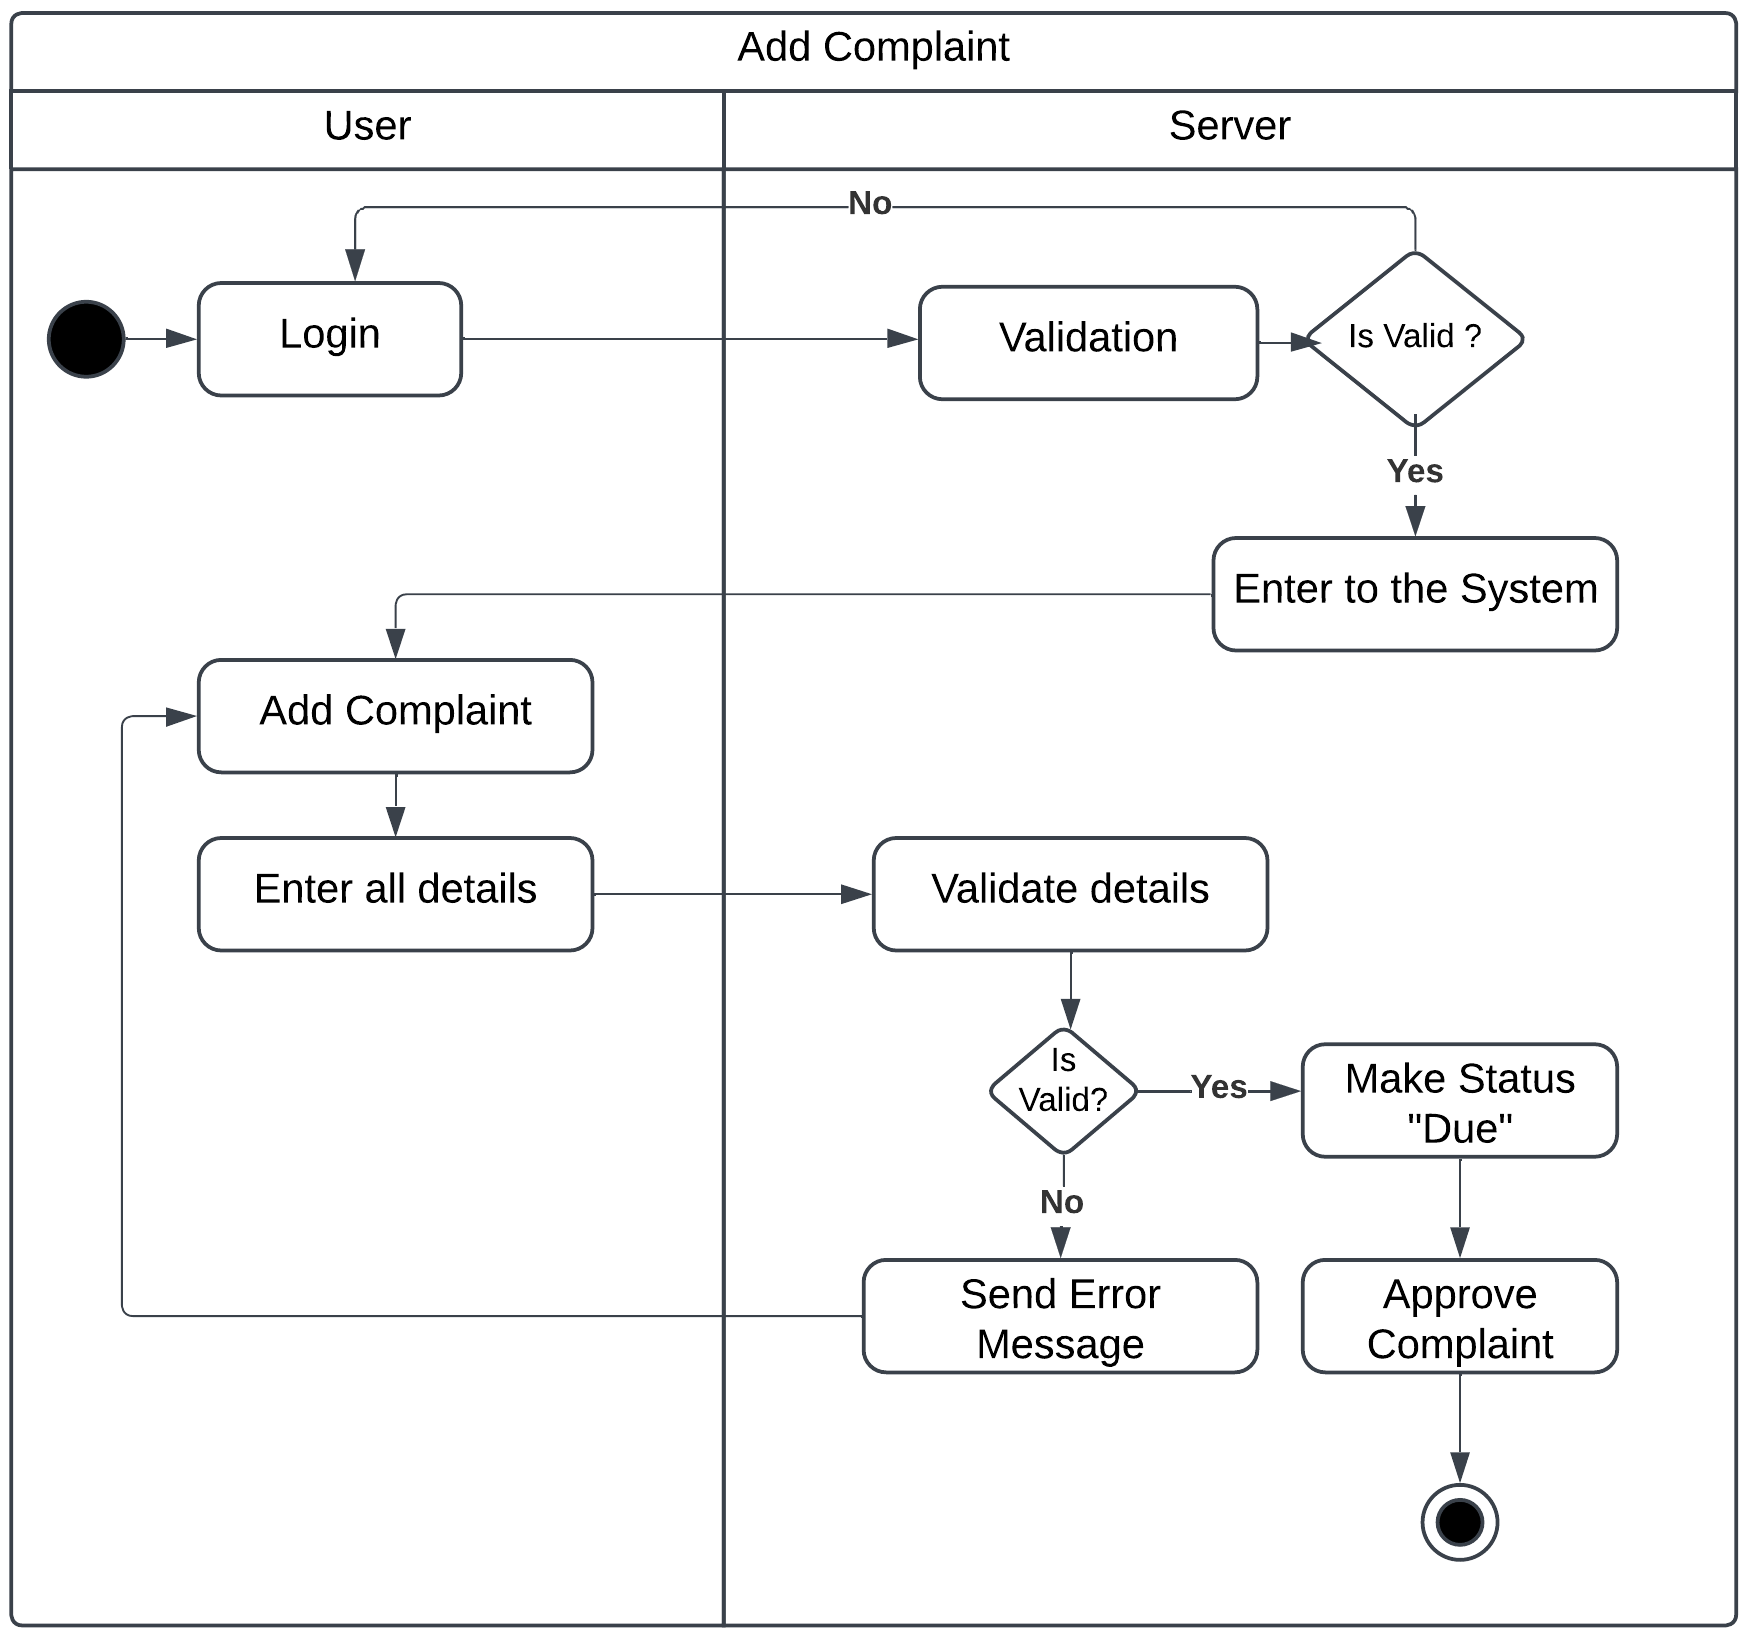
\includegraphics[width=1\linewidth]{photos/add-complain-activity-diagram.png}

    \caption{Activity Diagram of Making Complain Process by User}
    \label{fig:enter-label}
\end{figure}

\noindent\textbf{(b) Activity Diagram of the Complaint Management Process by Admin}
\begin{figure}[H]
    \centering
    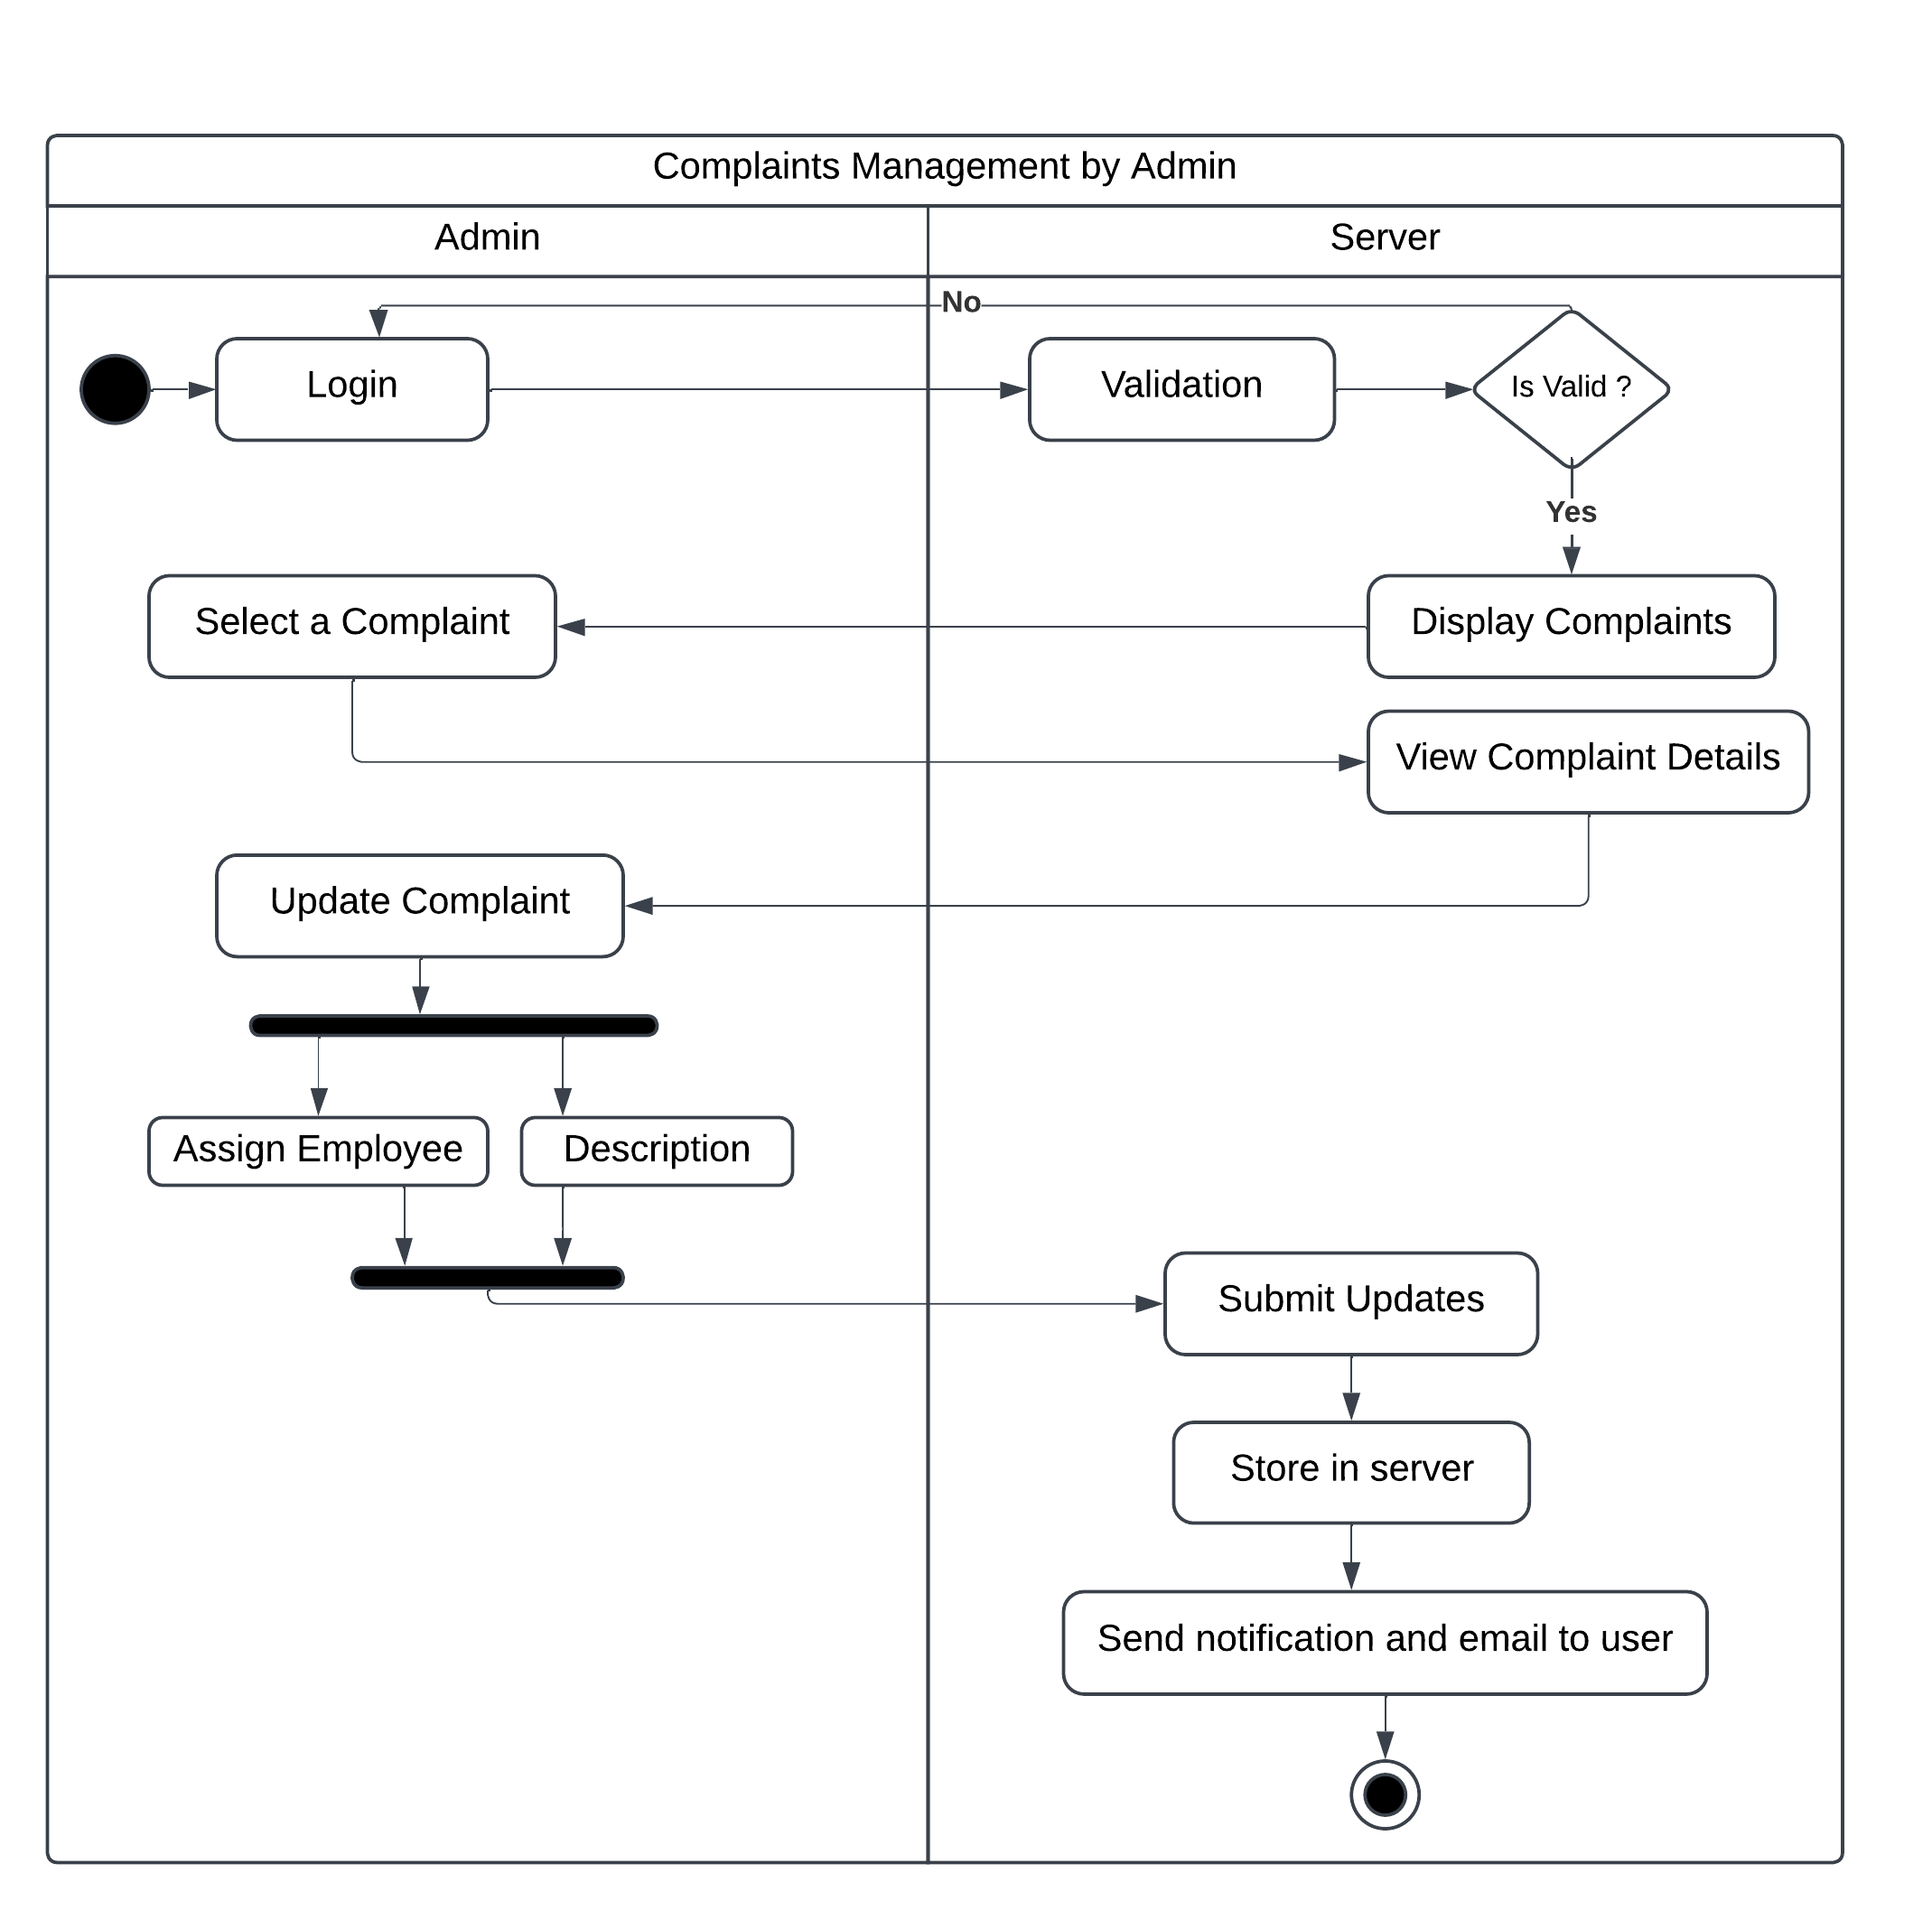
\includegraphics[width=1\linewidth]{photos/complaint-management-activity-diagram.png}

    \caption{Activity Diagram of Complaint Management Process by Admin}
    \label{fig:enter-label}
\end{figure}

\subsubsection{Sequence Diagram}
The Sequence Diagram illustrates the interaction between system components for two important processes, showing the order of messages exchanged between the objects in the system.

\noindent\textbf{(a) Sequence Diagram of Registration Process}
\begin{figure}[H]
    \centering
    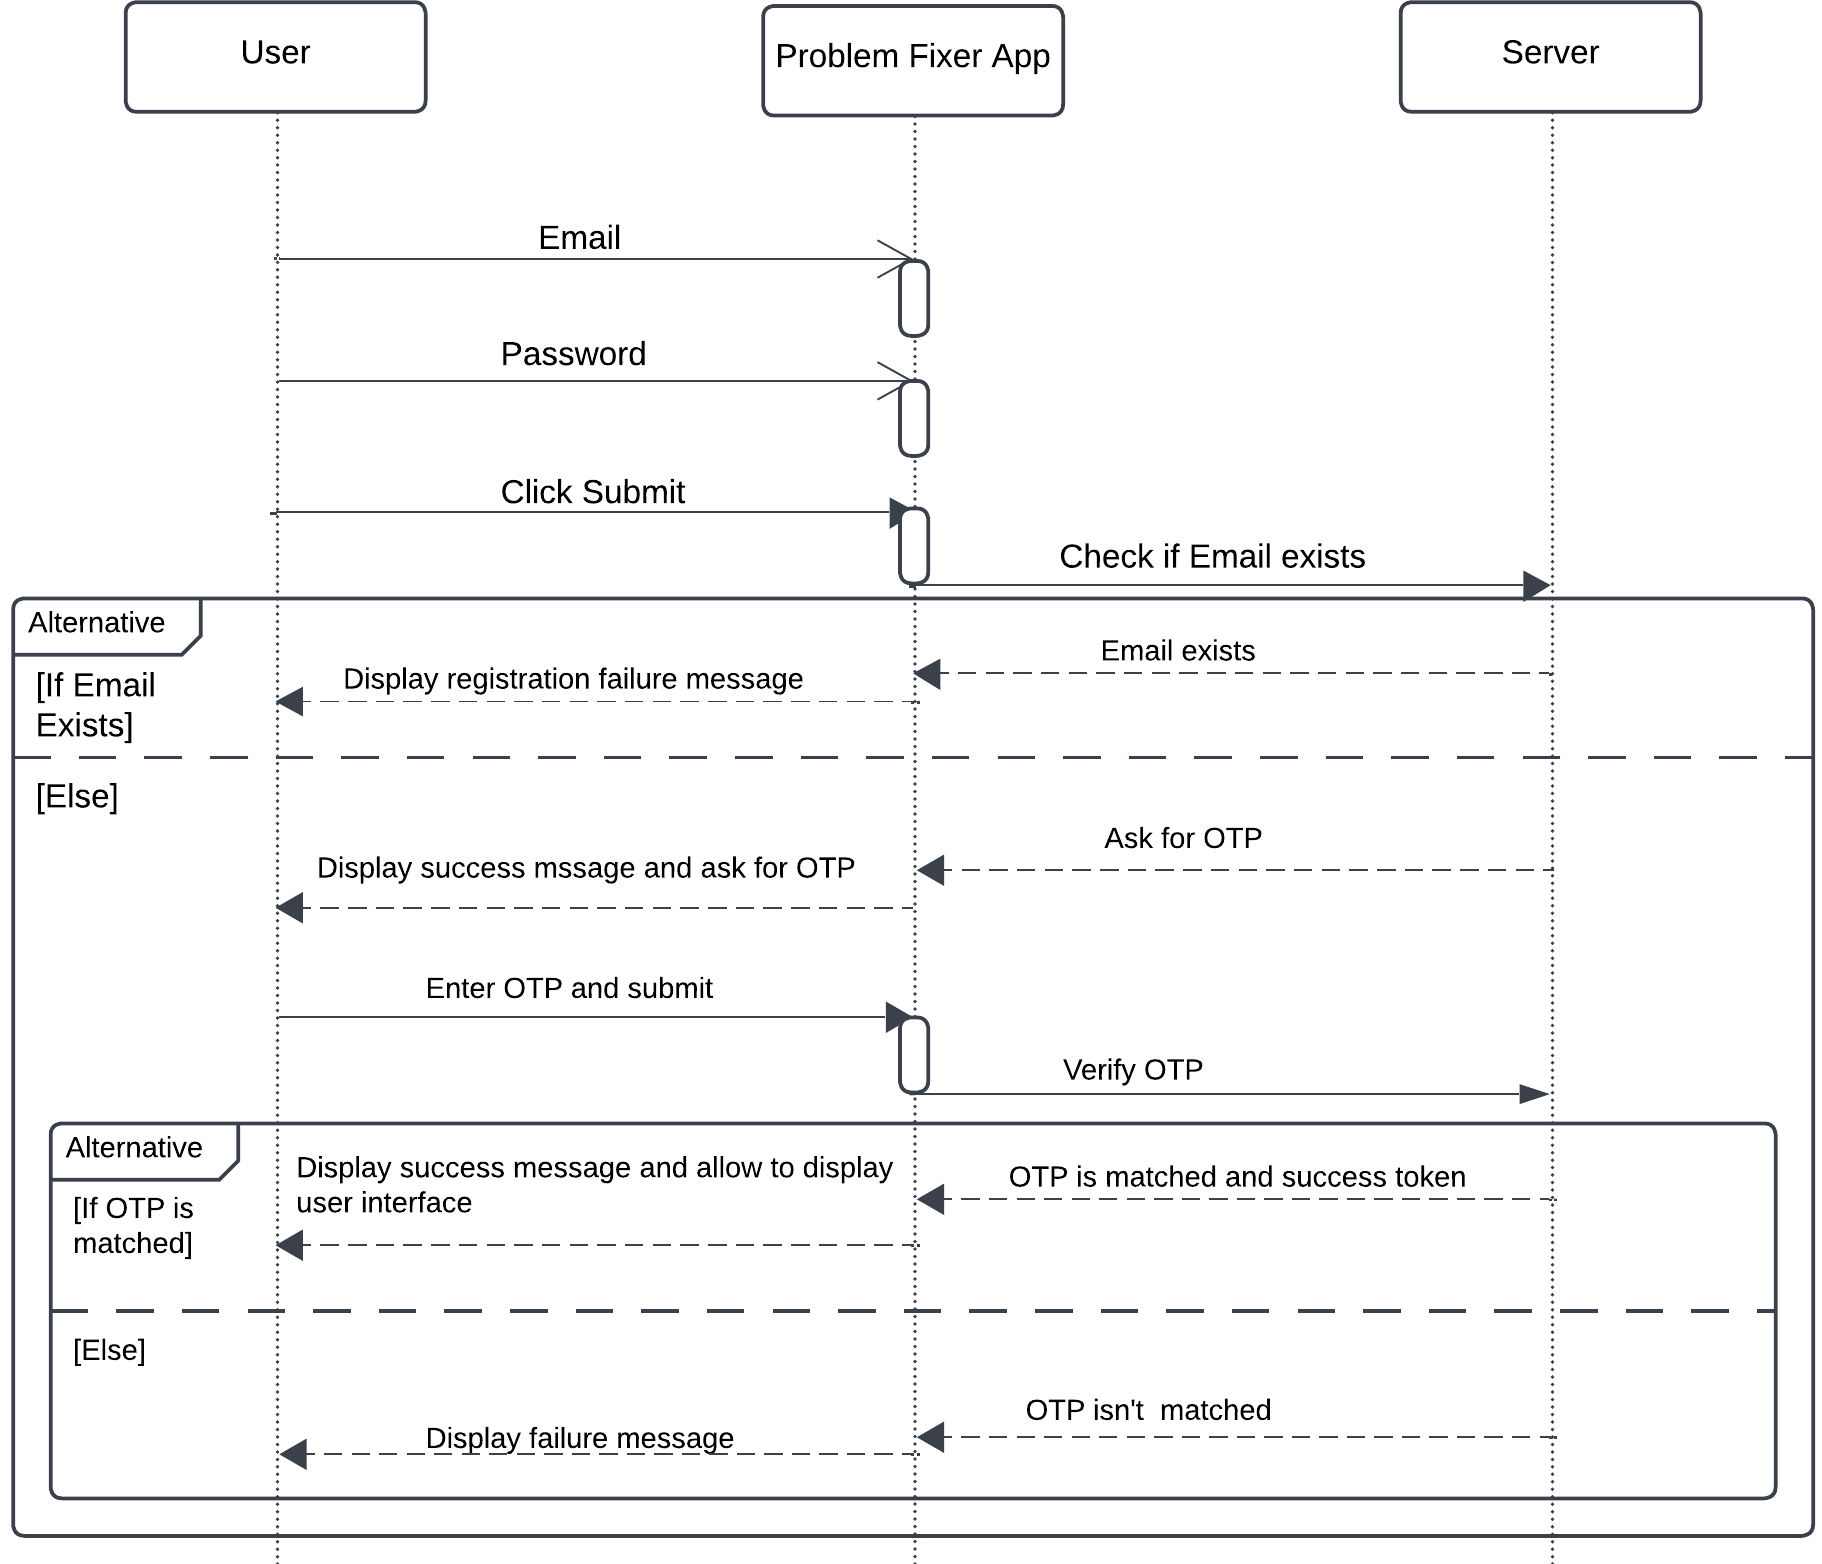
\includegraphics[width=1\linewidth]{photos/Registration-sequence-diagram.png}

    \caption{Sequence Diagram of Registration Process}
    \label{fig:enter-label}
\end{figure}
\noindent\textbf{(b) Sequence Diagram of Adding Employee}
\begin{figure}[H]
    \centering
    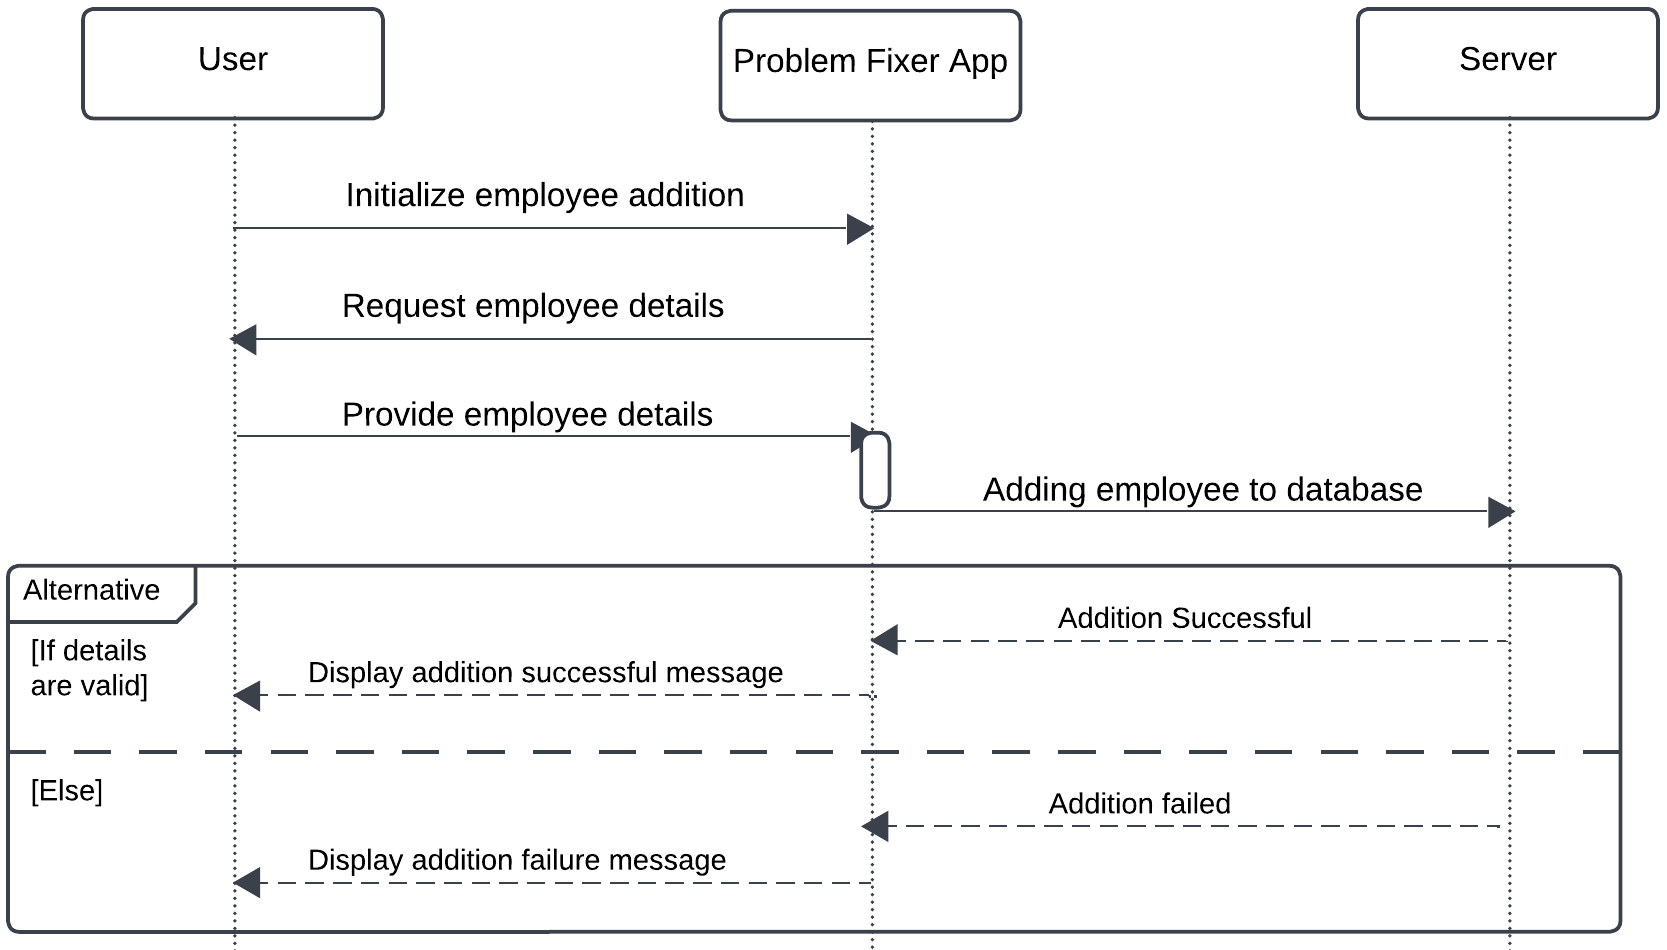
\includegraphics[width=1\linewidth]{photos/employee-sequence.png}

    \caption{Sequence Diagram of Adding Employee}
    \label{fig:enter-label}
\end{figure}

\subsection{Flow Models}
Flow models represent how data and control flow through the system, providing a clear picture of data processing and transformation.

\subsubsection{Level 0 DFD}
The Level 0 Data Flow Diagram (DFD) provides an overview of the system’s data flow and high-level processes. It represents the system as a single process, showing interactions with external entities and data inputs/outputs.
\begin{figure}[H]
    \centering
    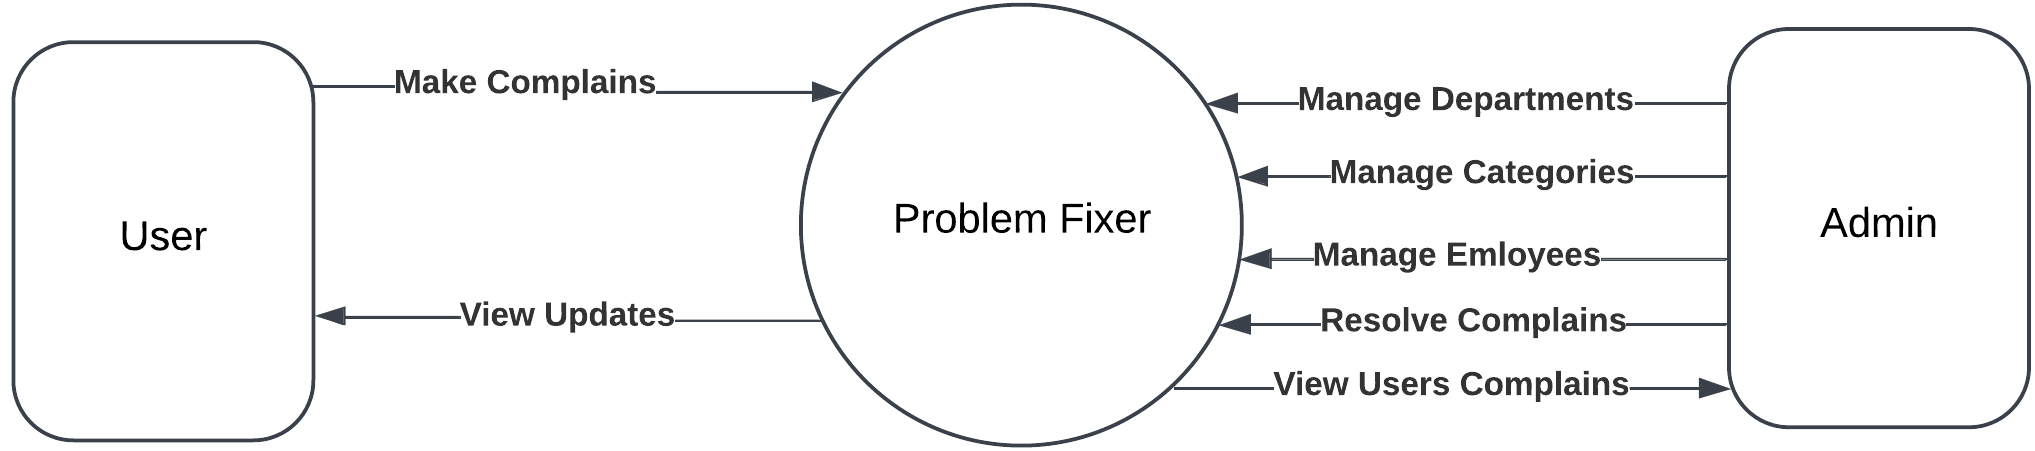
\includegraphics[width=1\linewidth]{photos/dfd-0.png}
    \caption{Sequence Diagram of Registration Process}
    \label{fig:enter-label}
\end{figure}

\subsubsection{Level 1 DFD}
The Level 1 DFD breaks down the major processes from the Level 0 DFD into more detailed components, illustrating how data flows within the system at a deeper level.
\begin{figure}[H]
    \centering
    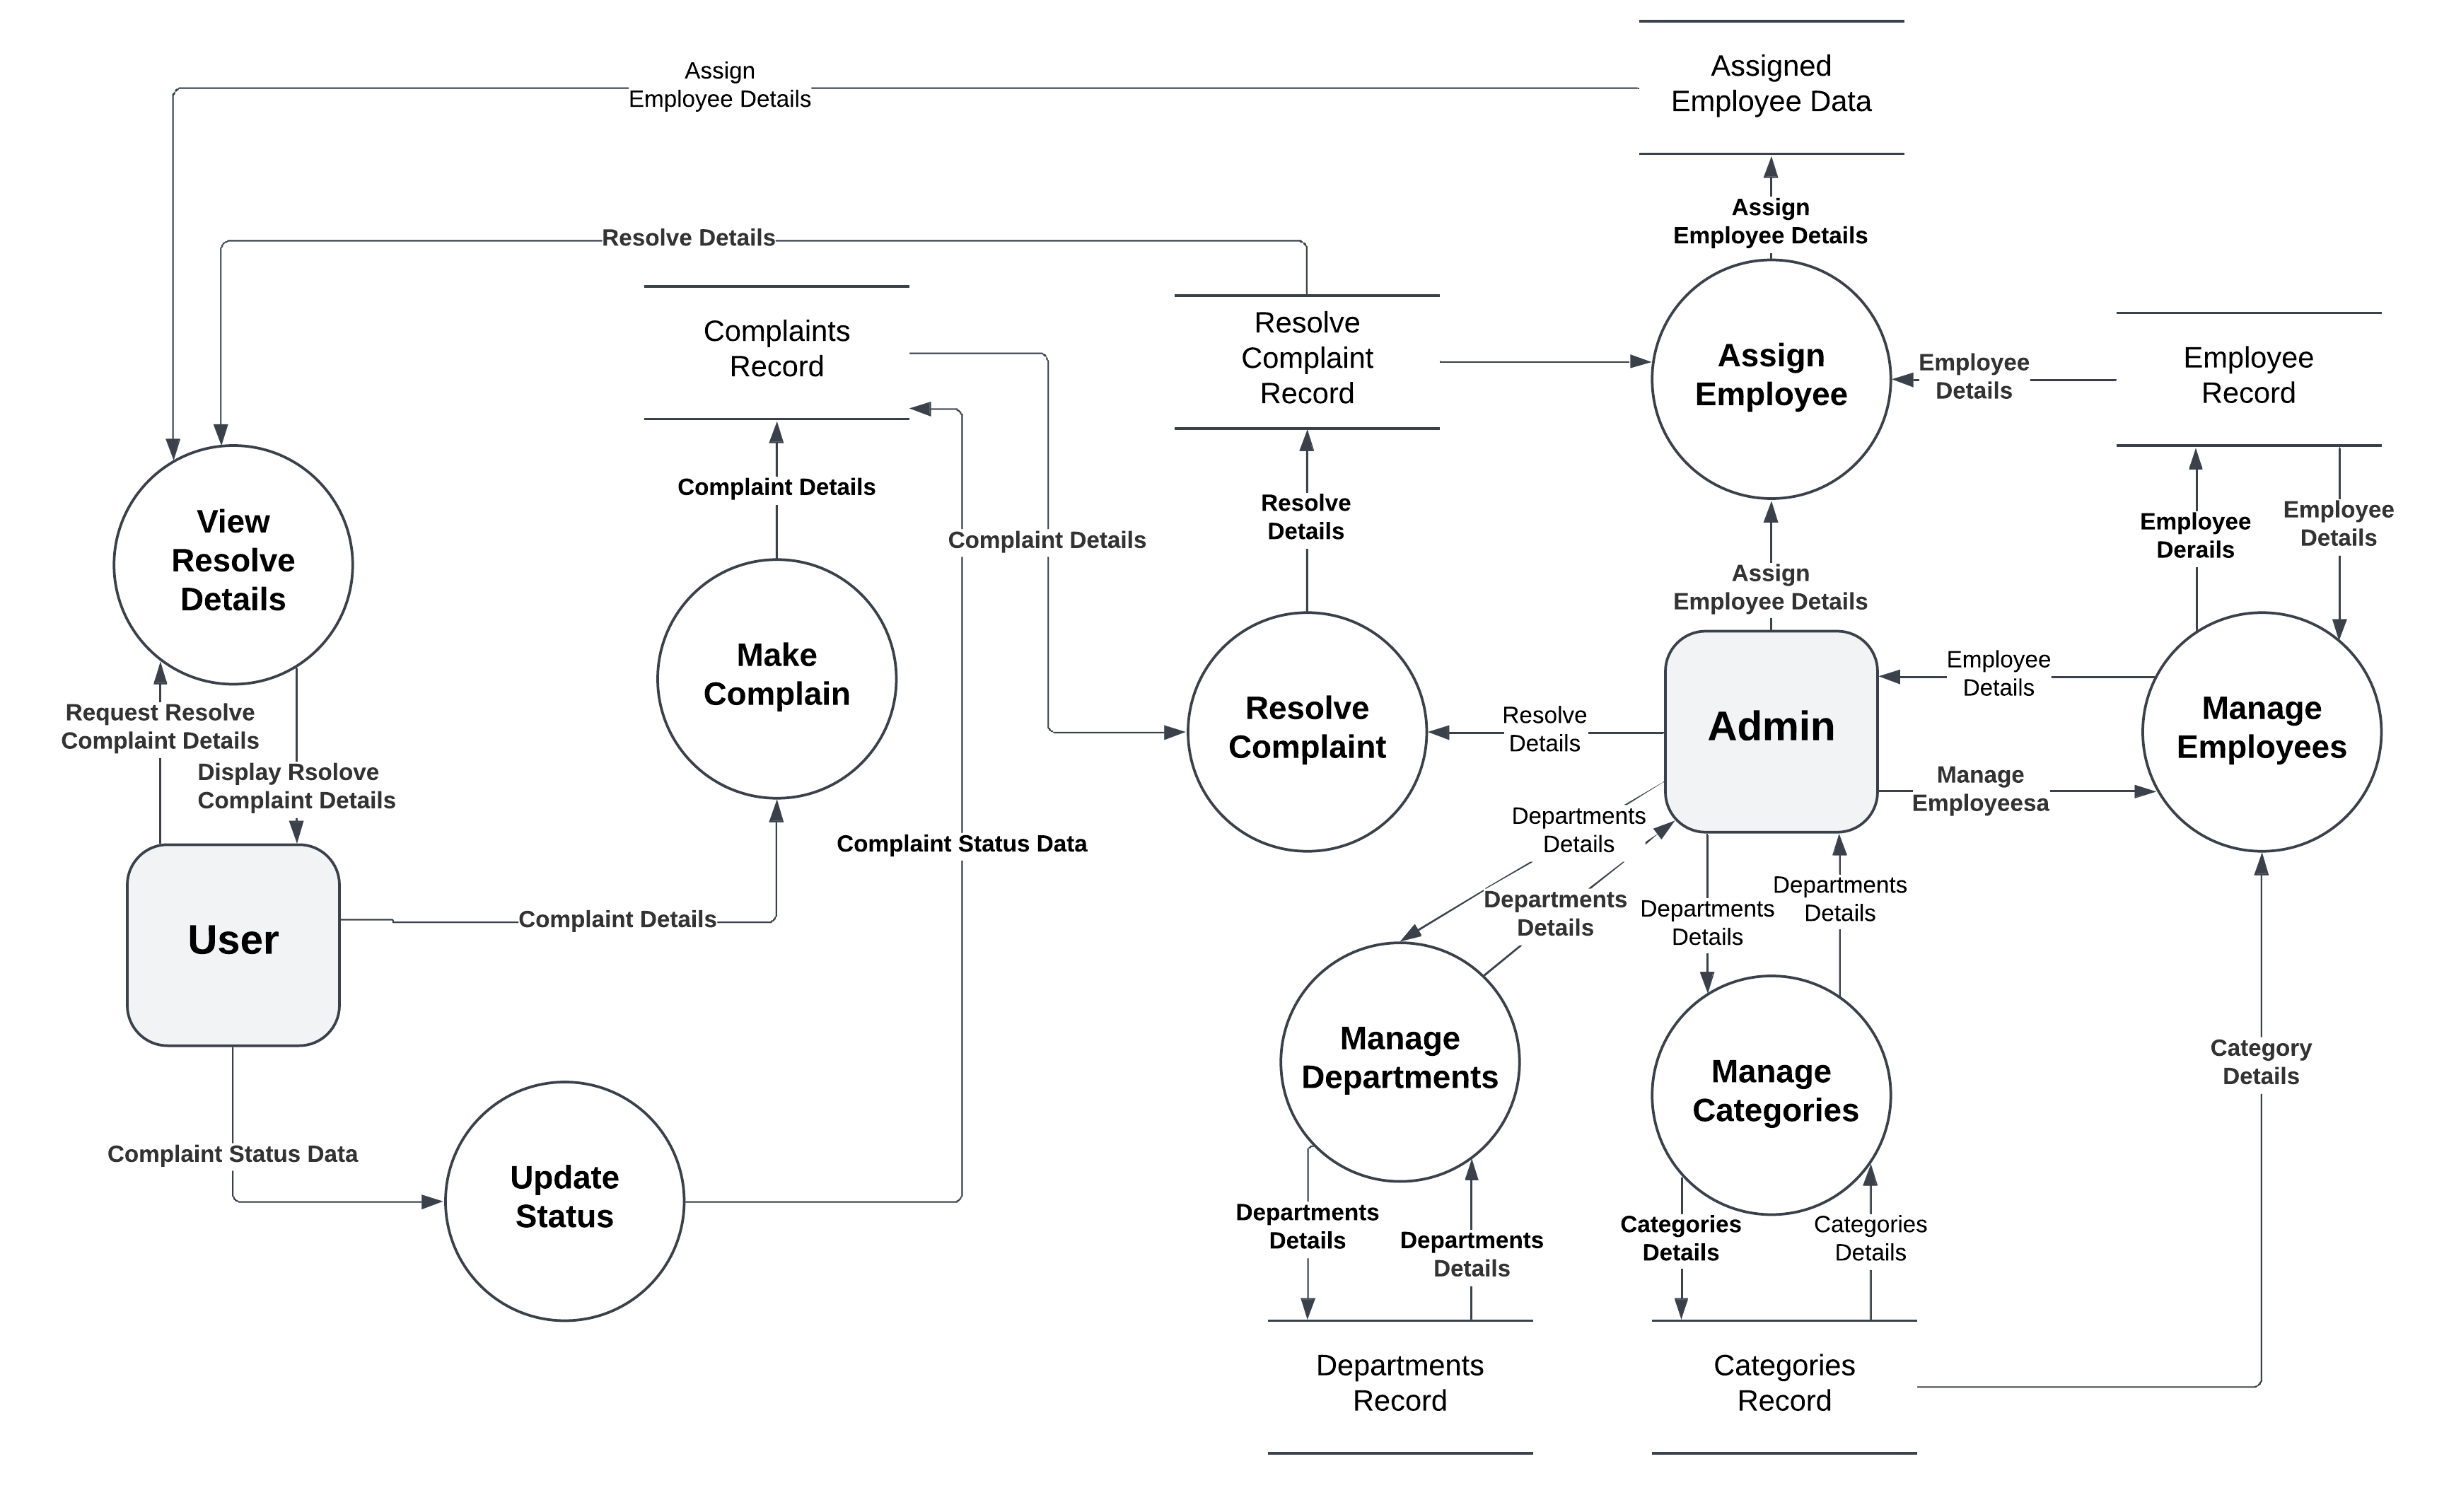
\includegraphics[width=1\linewidth]{photos/dfd-1.png}
    \caption{Sequence Diagram of Registration Process}
    \label{fig:enter-label}
\end{figure}
\end{document}
